\documentclass[a4paper]{article}
\usepackage[english]{babel}
\usepackage[a4paper,top=2cm,bottom=2cm,left=2cm,right=2cm,marginparwidth=1.75cm]{geometry}
\usepackage{amsmath}
\usepackage{amsfonts}
% \usepackage{amsthm}
\usepackage{amssymb}
\usepackage{graphicx}
\usepackage[colorinlistoftodos]{todonotes}
\usepackage[colorlinks=true, allcolors=blue]{hyperref}
\usepackage{import}
\usepackage{pdfpages}
\usepackage{transparent}
\usepackage{xcolor}
\usepackage{algorithmicx}
\usepackage{algpseudocode}
\usepackage{hyperref}

\usepackage{thmtools}
\usepackage{enumitem}
\usepackage[framemethod=TikZ]{mdframed}

\usepackage{xpatch}

\usepackage{boites}
\makeatletter
\xpatchcmd{\endmdframed}
{\aftergroup\endmdf@trivlist\color@endgroup}
{\endmdf@trivlist\color@endgroup\@doendpe}
{}{}
\makeatother

%\usepackage[poster]{tcolorbox}
%\allowdisplaybreaks
%\sloppy

\usepackage[many]{tcolorbox}

\xpatchcmd{\proof}{\itshape}{\bfseries\itshape}{}{}

% to set box separation
\setlength{\fboxsep}{0.8em}
\def\breakboxskip{7pt}
\def\breakboxparindent{0em}

\newenvironment{proof}{\begin{breakbox}\textit{Proof.}}{\hfill$\square$\end{breakbox}}
\newenvironment{ans}{\begin{breakbox}\textit{Answer.}}{\end{breakbox}}
\newenvironment{soln}{\begin{breakbox}\textit{Solution.}}{\end{breakbox}}

% \tcolorboxenvironment{proof}{
%     blanker,
%     before skip=\topsep,
%     after skip=\topsep,
%     borderline={0.4pt}{0.4pt}{black},
%     breakable,
%     left=12pt,
%     right=12pt,
%     top=12pt,
%     bottom=12pt,
% }
%
% \tcolorboxenvironment{ans}{
%     blanker,
%     before skip=\topsep,
%     after skip=\topsep,
%     borderline={0.4pt}{0.4pt}{black},
%     breakable,
%     left=12pt,
%     right=12pt,
% }

\mdfdefinestyle{enclosed}{
    linecolor=black
    ,backgroundcolor=none
    ,apptotikzsetting={\tikzset{mdfbackground/.append style={fill=gray!100,fill opacity=.3}}}
    ,frametitlefont=\sffamily\bfseries\color{black}
    ,splittopskip=.5cm
    ,frametitlebelowskip=.0cm
    ,topline=true
    ,bottomline=true
    ,rightline=true
    ,leftline=true
    ,leftmargin=0.01cm
    ,linewidth=0.02cm
    ,skipabove=0.01cm
    ,innerbottommargin=0.1cm
    ,skipbelow=0.1cm
}

\mdfsetup{%
    middlelinecolor=black,
    middlelinewidth=1pt,
roundcorner=4pt}

\setlength{\parindent}{0pt}

\mdtheorem[style=enclosed]{theorem}{Theorem}
\mdtheorem[style=enclosed]{lemma}{Lemma}[theorem]
\mdtheorem[style=enclosed]{claim}{Claim}[theorem]
\mdtheorem[style=enclosed]{ques}{Question}
\mdtheorem[style=enclosed]{defn}{Definition}
\mdtheorem[style=enclosed]{notn}{Notation}
\mdtheorem[style=enclosed]{obs}{Observation}
\mdtheorem[style=enclosed]{eg}{Example}
\mdtheorem[style=enclosed]{cor}{Corollary}
\mdtheorem[style=enclosed]{note}{Note}

% \let\thetheorem=\relax
% \let\thelemma=\relax
% \let\theclaim=\relax
% \let\theques=\relax
% \let\thedefn=\relax
% \let\thenotn=\relax
% \let\theobs=\relax
% \let\thecor=\relax
% \let\thenote=\relax

% \renewcommand\qedsymbol{$\blacksquare$}
\newcommand{\nl}{\vspace{0.2cm}\\}
\newcommand{\ol}{\overline}
\newcommand{\eps}{\varepsilon}
\newcommand{\mc}{\mathcal}
\newcommand{\mi}{\mathit}
\newcommand{\mf}{\mathbf}
\newcommand{\mb}{\mathbb}
\newcommand{\R}{\mathbb{R}}
\newcommand{\Z}{\mathbb{Z}}
\newcommand{\OPT}{\mathbf{OPT}}
\newcommand{\ALG}{\mathbf{ALG}}
\renewcommand{\L}{\mc{L}}
\newcommand{\changesto}{\vdash}
\newcommand\Vtextvisiblespace[1][.3em]{%
    \mbox{\kern.06em\vrule height.3ex}%
    \vbox{\hrule width#1}%
    \hbox{\vrule height.3ex}
}
\newcommand{\blank}{{\Vtextvisiblespace[0.7em]}}
\newcommand{\leftend}{\triangleright}
\newcommand{\comp}{\overline}

\newcommand{\incfig}[1]{%
    \def\svgwidth{\columnwidth}
    \import{./figures/}{#1.pdf_tex}
}
\pdfsuppresswarningpagegroup=1

\title{\textbf{ELL888 Minor Exam}}
\author{Navneel Singhal, 2018CS10360}
\date{}

\begin{document}

\maketitle
\tableofcontents

\section{Graph learning setting}

You are given $\mf{X} \in \R^{n \times d}$ whose rows reside on the vertices of an unknown graph.
\begin{align*}
    X = \begin{bmatrix}
        - \mf{x}_1 \in \R^d -\\
        - \mf{x}_2 \in \R^d -\\
            \mid \\
        - \mf{x}_n \in \R^d -\\
    \end{bmatrix}
\end{align*}
Graph learning from data simply means finding an edge-weight matrix $\mf{A} \in \R^{n \times n}$ where its element $w_{ij} = {[A]}_{ij}$ captures the relation between any two pairs of vertices $(i,
j)$, i.e., data points $(\mf{x}_i, \mf{x}_j)$. We learn the graph weights $\mf{w} \in \R^{n(n - 1)/2}$ under certain assumptions like smoothness, probabilistic distribution, nearest
neighbourhood, etc. The focus here is an undirected graph which implies that the graph matrix is symmetric. Now consider the following problems.

\section{Graph learning with missing data}

\subsection{Problem}
\begin{align*}
    X = \begin{bmatrix}
        \mf{x}_1 = [x_{11}, x_{12}, \bullet, x_{14}, \ldots, x_{1d}]\\
        \mf{x}_2 = [x_{21}, \bullet, x_{23}, \bullet, x_{25}, \ldots, x_{1d}]\\
        \mid\\
        \mf{x_n} = [\bullet, x_{n2}, \bullet, x_{n4}, \ldots, x_{nd}]
    \end{bmatrix}
\end{align*}
where some parts of the data are missing at random and $\bullet$ indicates missing data. Explain in detail how we can learn the graph matrix with missing data (in descriptive detail).

\subsection{Solution}
I will mainly focus on solving this problem under smoothness constraints --- i.e., I will assume that we want to learn a graph from a smooth signal.

\subsubsection{Optimization problem formulation}
Firstly, note that a rudimentary imputation scheme is to do the following: for each feature $i \in \{1, \ldots, d\}$, let $D$ be the distribution of the values for the feature that are not
missing. Then, for each $x_i$ such that $x_{id}$ is a missing feature, assign to it a value sampled from $D$. We could also assign it something different --- for instance, the mean of $D$.\nl
However, this is clearly not good enough. Let's look at the formulation of the optimization problem for the weights $\mf{w}$ (with $w(i, j)$ corresponding to the weight of the edge between
$i$ and $j$). It looks something like the following:\\
\begin{align*}
    \min_{w} \sum_{1 \le i < j \le n} w(i, j) ||\mf{x}_i - \mf{x}_j||_2^2\\
    \text{subject to certain constraints on }w
\end{align*}
Note that we are working under the assumption that the signal is smooth. Considering the fact that in graph regularization, such an ``energy'' term is used to penalize the objective function, it
makes sense to consider the above problem as a minimization problem when we vary the missing data as well, so as to ensure that the graph signal is indeed smooth. That is, the problem transforms to the following:

\begin{align*}
    \min_{w, x_{\text{unknown}}} \sum_{1 \le i < j \le n} w(i, j) ||\mf{x}_i - \mf{x}_j||_2^2\\
    \text{subject to certain constraints on }w
\end{align*}

In a sense, alongside the weights $\mf{w}$, we are also learning the missing data under the smoothness assumption.

\subsubsection{Solving the optimization problem}
For solving this optimization problem, we can follow the following iterative method to solve for optimal $w, x_{\text{unknown}}$ given that we have a solver for the original problem as a
black-box (in certain special cases, it is possible to solve this directly rather than relying on the following distribution):

\begin{enumerate}
    \item For each feature $j \in \{1, \ldots, d\}$, compute the multiset $D_j$ of values that appear in $\mf{X}$, and for each $\mf{x}_i$ such that $x_{ij}$ is missing, assign
        to $x_{ij}$ a random sample from $D_j$ (or the mean).
    \item Until a stopping condition is reached, do the following:
        \begin{itemize}
            \item Keeping $x_{\text{unknown}}$ fixed, solve the optimization problem for $\mf{w}$ using the black-box algorithm.
            \item Keeping $\mf{w}$ fixed, solve the quadratic programming problem for $x_{\text{unknown}}$ to get an optimal solution $x^*_{\text{unknown}}$.
        \end{itemize}
    \item Return the learned weights $\mf{w}$.
\end{enumerate}

Here, the first step tries to learn $\mf{w}$ using our prior beliefs about the unknown data, and later on, we try to refine the unknown data by performing some sort of regularization of the
graph signal in order to fit it to a more regular signal.\nl

Note that if a fraction $k$ of the data was missing, then in the quadratic programming problem that we need to solve, there would be $knd$ variables, which might be infeasible for a
large number of variables. A variant of the above method would be to optimize over these unknown variables in batches (similar to stochastic gradient descent) while keeping the other variables
constant, so as to make the size of this problem small enough.

\subsubsection{Experiments using some standard techniques}
Firstly, a comment on the applicability of this method: note that in the mentioned algorithm, we assumed that we only have access to an oracle that learns weights from a graph (and it is called in
the second part of the loop in our algorithm). Hence, this method is applicable for practically any scenario where we want to learn the weight matrix from data, no matter what the constraints
on $\mf{w}$ that the oracle provides, or the form of the objective function (though if the dependence of the objective function on $x$ is not quadratic, it becomes a different problem ---
however, the idea remains the same). However, it is not clear if the convergence is guaranteed.\nl
To benchmark it, we shall use the approach in the following paper for the aforementioned oracle:

\begin{itemize}
    \item Dong et al. ``Laplacian Matrix Learning for Smooth Graph Signal Representation''. ICASSP, 2015.
\end{itemize}

Since our objective at hand is to see how well the imputed data represents the original data had it not been missing, we shall take the following approach:
\begin{itemize}
    \item Take a dataset $X$ of complete data, and remove a certain fraction of values to get a new dataset $X'$.
    \item Using the oracle $\mc{O}$, compute the graph $G$, and using our algorithm, compute the graph $G'$ and the dataset $X''$ consisting of new values.
    \item Compute the difference between $X$ and $X''$ on the imputed parts for each feature, and find the average square of the difference between the actual data and imputed data for each
        feature.
    \item Compare the F-measures of edge existence.
\end{itemize}

Since we are working under the assumption that the graph signal is smooth, we will choose the following dataset:

\begin{itemize}
    \item Randomly generated sensor networks: Since sensor networks aim to measure some physical property, which should be reasonably smooth, these graphs are good candidates for this approach.
        The graph signal is generated by embedding these sensors in 2D and applying smooth functions to their coordinates.
\end{itemize}

The implementation uses the base code found at \href{https://github.com/rodrigo-pena/graph-learning}{https://github.com/rodrigo-pena/graph-learning}, and it was retrieved from
\href{https://paperswithcode.com/paper/how-to-learn-a-graph-from-smooth-signals}{https://paperswithcode.com/paper/how-to-learn-a-graph-from-smooth-signals}. Some of the metrics that we
want are already implemented there, but we used new metrics and they are self-implemented.\nl

For the following experiments, we have $n = 256, d = 4$. In the baseline, we assign the mean of the feature to the missing values. We use $k = 0.05$ and $k = 0.1$ (i.e., $5\%$ and $10\%$ of data
missing respectively) in two independent sets of experiments to show the differences between this and the baseline.

Define $$\ell_j = \sqrt{\frac{\sum_{i = 1}^n (x_{ij} - x_{ij, \text{imputed}})^2}{\sum_{i = 1}^n 1_{x_{ij}\text{ is missing}}}}$$

and
$$
\omega = \frac{||W_{full} - W_{imputed}||_F^2}{n \times d}
$$

Then we have the following

\begin{center}
\begin{tabular}{|c|c|c|c|}
    \hline
                                & Baseline  & Our algorithm     & No missing data \\
    \hline
    F2-score at $k = 0.05$      & 0.60      & 0.67              & 0.70 \\
    \hline
    F2-score at $k = 0.1$       & 0.49      & 0.61              & 0.69 \\
    \hline
    $\omega$ at $k = 0.05$      & 0.0165    &    0.0118         & ---\\
    \hline
    $\omega$ at $k = 0.1$       & 0.0357    &    0.0223         & ---\\
    \hline
    $\ell_1$ at $k = 0.05$      & 1.156     &    0.833          & ---\\
    \hline
    $\ell_2$ at $k = 0.05$      & 4.033     &      3.894          & ---\\
    \hline
    $\ell_3$ at $k = 0.05$      & 1.875     &      1.715        & ---\\
    \hline
    $\ell_4$ at $k = 0.05$      & 0.971     &      0.5712        & ---\\
    \hline
    $\ell_1$ at $k = 0.1$       & 1.359     &    0.956         & ---\\
    \hline
    $\ell_2$ at $k = 0.1$       & 2.558     &   2.1034           & ---\\
    \hline
    $\ell_3$ at $k = 0.1$       & 1.778     &    1.745         & ---\\
    \hline
    $\ell_4$ at $k = 0.1$       & 0.910     &    0.770          & ---\\
    \hline

\end{tabular}
\end{center}

\begin{center}
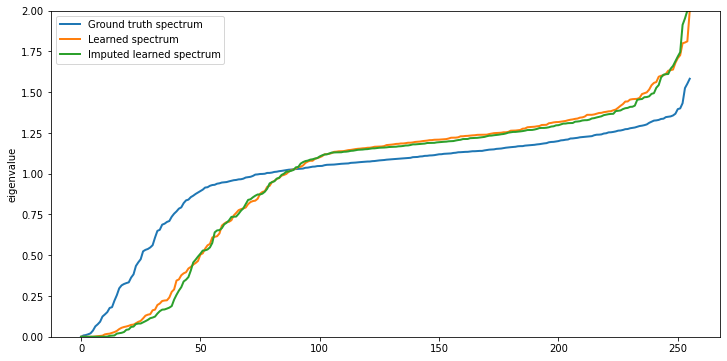
\includegraphics[width=0.70\textwidth]{images/5_percent_own_spectrum.png}\\
Spectrum for $k = 0.05$\\
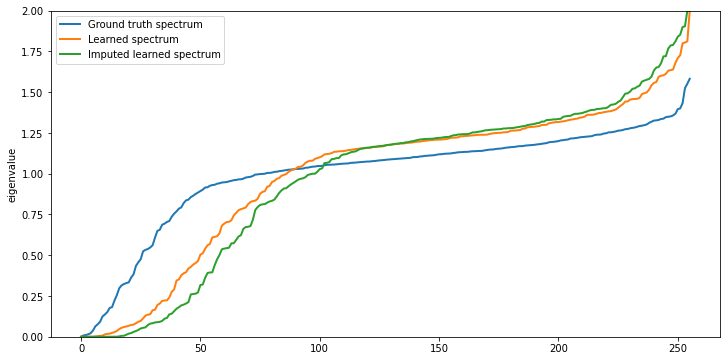
\includegraphics[width=0.70\textwidth]{images/5_percent_baseline_spectrum.png}\\
Baseline spectrum for $k = 0.05$\\
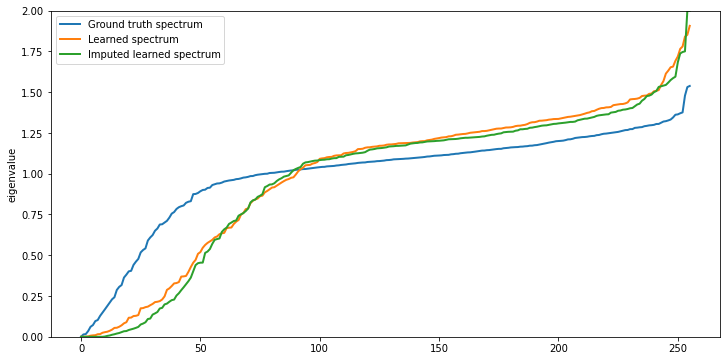
\includegraphics[width=0.70\textwidth]{images/10_percent_own_spectra.png}\\
Spectrum for $k = 0.1$\\
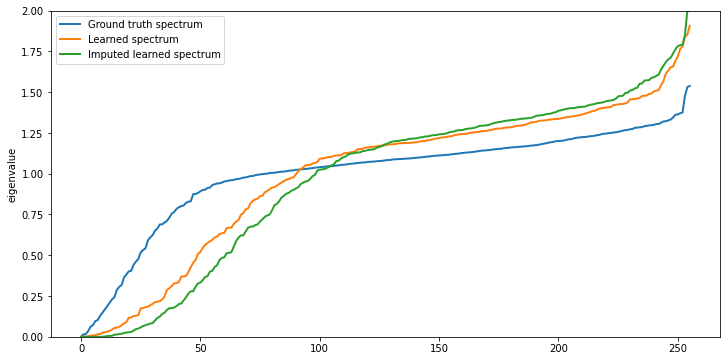
\includegraphics[width=0.70\textwidth]{images/10_percent_baseline_spectra.png}\\
Baseline spectrum for $k = 0.1$\\
\end{center}

As we can see in the above plots of the eigenvalues, our algorithm matches the eigenvalues fairly well.

Now we will show how the learned graphs look like (for $k = 0.1$, baseline and our algorithm respectively):

\begin{center}
    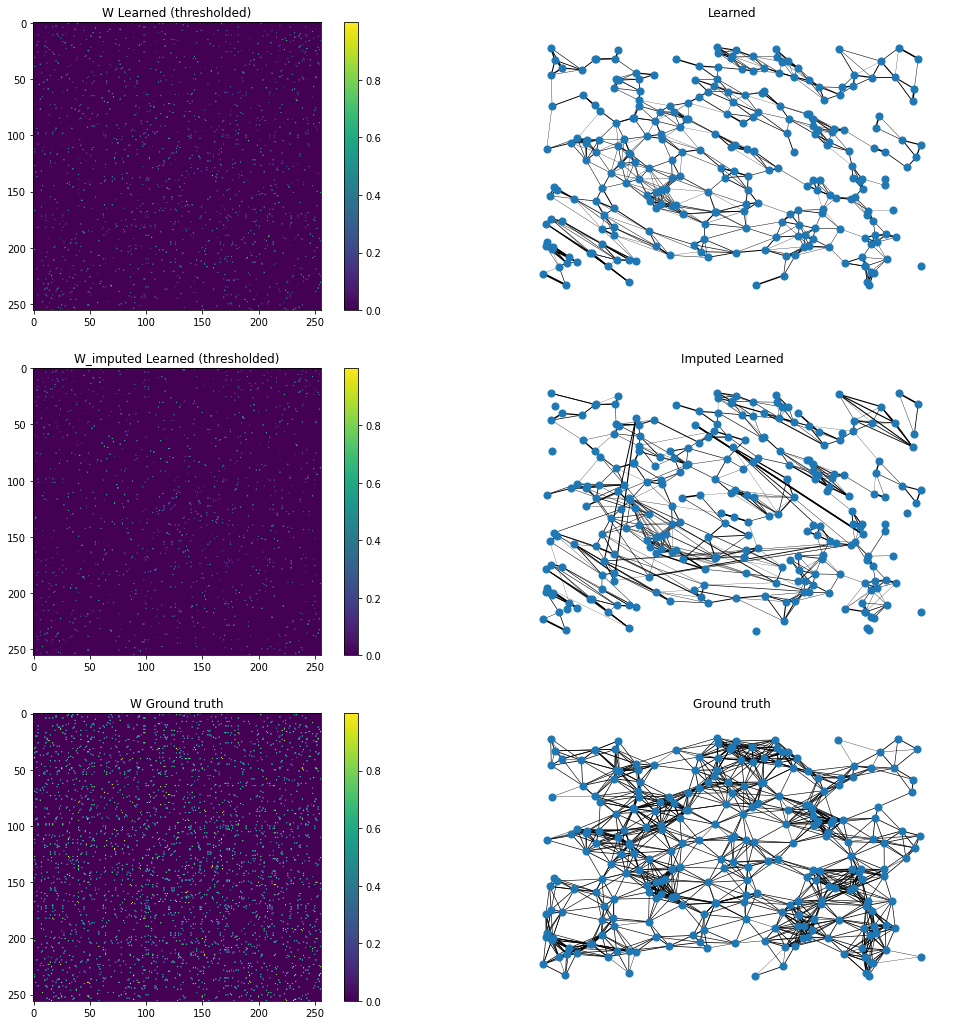
\includegraphics[width=0.45\textwidth]{images/10_percent_baseline_learned_graphs.png}
    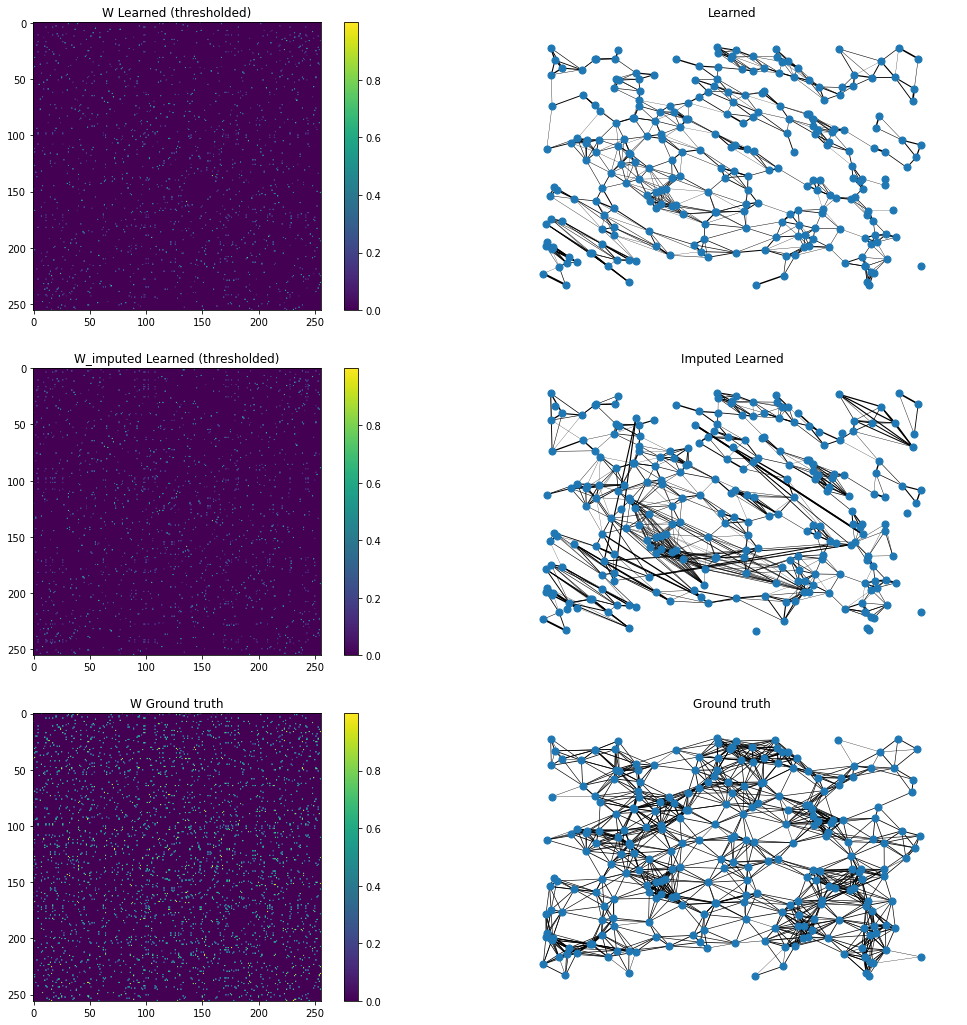
\includegraphics[width=0.45\textwidth]{images/10_percent_own_learned_graphs.png}
\end{center}

\newpage

\section{Semi-supervised setting}

\subsection{Problem}

Now consider a semi-supervised graph learning problem. With the data $\mf{X}$ sitting at $n$ vertices, we also have the label information for $k < n$ vertices. Simply, we have $\mf{X} \in \R^{n \times
d}$ with label information for $k$ vertices $\mf{y} \in \{0, 1\}^k$. Explain in detail how can we learn the graph matrix integrating the label information. The dataset available is
$\left(\{\mf{x}_i, y_i\}_{i = 1}^k, \{\mf{x}_j\}_{j = k + 1}^n\right)$.

\subsection{Solution}

\section{Massive data setting}

\subsection{Problem}

Consider a massive data scenario, where $n$ and $d$ both are very large, and typically $n \gg d$. It is not possible to process the entire data every iteration. Explain how we can approach
the graph learning problem under such a setting. (Hint: Stochastic gradient descent based approaches try to address such problems, where each iteration is performed considering only a small
subset of the dataset, or a \emph{minibatch}).

\subsection{Solution}


\section{Heterogeneous data scenario}

\subsection{Problem}

Consider a heterogeneous data scenario, where the dataset $\mf{X}$ associated with vertices may belong to the set of reals $\R$, the set of integers $\mb{I}$, and categorical $\mb{C} = \{c_1,
\ldots, c_k\}$. More concretely, $\mf{X} \in \R^{n \times d_r} \times \mb{I}^{n \times d_i} \times \mb{C}^{n \times d_c}$ and $d = d_r + d_i + d_c$. For example, $\mf{x}_1 = [x_{11}, x_{12},
\ldots, x_{1d_r} \in \R, x_{1(d_r + 1)}, x_{1(d_r + 2)}, \ldots, x_{1(d_r + d_i)} \in \mb{I}, x_{1(d_r + d_i + 1)}, d_{1(d_r + d_i + 2)}, \ldots, x_{1(d_r + d_i + d_c)} \in \mb{C}]$. Explain in
detail how we can learn a graph matrix with heterogeneous data setting (in descriptive detail).

\subsection{Solution}


\end{document}
